\section{What we discussed last time}
\subsection{Model Architectures}
\begin{frame}{Model Architecture Separate Tails}
	\centering
	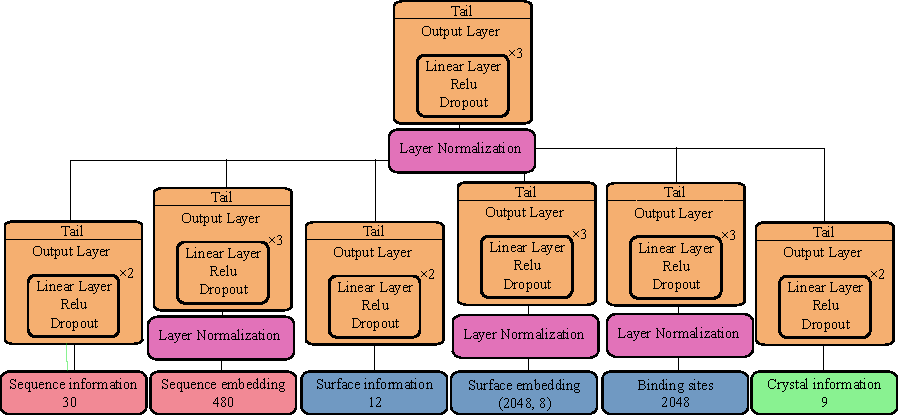
\includegraphics[width=0.95\linewidth]{media/modelArchitectureSeparateTails}
\end{frame}

\begin{frame}{Model Architecture Joined Tail}
	\centering
	
\includegraphics[width=0.95\linewidth]{media/modelArchitectureJoinedTail
	}
\end{frame}

\subsection{Performance on Ph Prediction task}
\begin{frame}{Performance on Ph Prediction task}	
	\begin{columns}[T,onlytextwidth]		
		\begin{column}{0.3\textwidth}
		\begin{itemize}
			\item Validation split 0.2 based on unique entry id similar to \citet{Lee2019}
			\item Explained Variance: 
			\begin{itemize}
				\item Train: 0.96
				\item Validation: 0.89
			\end{itemize}
			\item Pearson: 
			\begin{itemize}
				\item Train: 0.98
				\item Validation: 0.9
			\end{itemize}
		\end{itemize}
		\end{column}
		
		% RIGHT COLUMN: boxtext
		\begin{column}{0.6\textwidth}			
			\begin{figure}
				\centering
				\includegraphics[width=1\linewidth]{../../msc-thesis-code/data/dataExploration/plots/RFPerformancePh}
			\end{figure}
		\end{column}		
		
	\end{columns}	
\end{frame}

\section{What has changed since then}
\subsection{Performance on Ph Prediction task}
\begin{frame}{Performance on Ph Prediction task with valid split}
	\begin{columns}[T,onlytextwidth]		
		\begin{column}{0.3\textwidth}
			\begin{itemize}
				\item \small protein based validation split instead of entry based
				\item \small build bi-partition tree to avoid data leakage from files with multiple proteins 
				\item Explained Variance: 
				\begin{itemize}
					\item Train: 0.96
					\item Validation: 0.25
				\end{itemize}
				\item Pearson: 
				\begin{itemize}
					\item Train: 0.98
					\item Validation: 0.5
				\end{itemize}
			\end{itemize}
		\end{column}
		
		
		\begin{column}{0.6\textwidth}			
			\begin{figure}
				\centering
				\includegraphics[width=1\linewidth]{../../msc-thesis-code/data/dataExploration/plots/split_corrected_ph_performance}
			\end{figure}
		\end{column}		
		
	\end{columns}	
\end{frame}


\subsection{Reasons for overfitting}
\begin{frame}{Performance on Ph Prediction task with valid split}
\begin{figure}[h!]
	\centering		
	\begin{subfigure}[t]{0.595\linewidth}
		\centering
		\includegraphics[width=\linewidth]{../../msc-thesis-code/data/dataExploration/plots/proteinEmbedding}
	\end{subfigure}
	\begin{subfigure}[t]{0.395\linewidth}
		\centering
		\includegraphics[width=\linewidth]{../../msc-thesis-code/data/dataExploration/plots/proteinDistributionpH_temp}
		\caption[pH sequence embedding]{Median and variance for Ph/Temperature for a given protein}
		\label{fig:pHEmbedding}
	\end{subfigure}
\end{figure}
\end{frame}


\subsection{Chemical prediction}
\begin{frame}{Prediction of chemicals}
	\begin{columns}[T,onlytextwidth]		
		\begin{column}{0.3\textwidth}
			\begin{itemize}
				\item multi-hot encode chemicals ([0, 0, 1, 1, 0, ..., 0, 1, 0])
				\item top 300 chemicals 
				\item for inference check for top 
			\end{itemize}
		\end{column}
		
		
		\begin{column}{0.6\textwidth}			
			\begin{figure}
				\centering
				\includegraphics[width=1\linewidth]{../../msc-thesis-code/data/dataExploration/plots/chemical_prediction_auroc_train_vs_val}
			\end{figure}
		\end{column}		
		
	\end{columns}	
\end{frame}

\begin{frame}{Prediction of chemicals}
	\begin{columns}[T,onlytextwidth]		
		\begin{column}{0.25\textwidth}
			\begin{itemize}
				\item Even for training the predictions are pretty bad 
				\item Model performance strongly biased towards often occurring chemicals	
			\end{itemize}
		\end{column}
		

		\begin{column}{0.7\textwidth}
			\vspace{-0.75cm}			
			\begin{figure}
				\centering
				\includegraphics[width=1\linewidth]{../../msc-thesis-code/data/dataExploration/plots/MissRateFpRate}
			\end{figure}
		\end{column}		
		
	\end{columns}	
\end{frame}

{ % all template changes are local to this group.
	\setbeamertemplate{navigation symbols}{}
	\begin{frame}<article:0>[plain]
		\begin{tikzpicture}[remember picture,overlay]
			\node[at=(current page.center)] {
				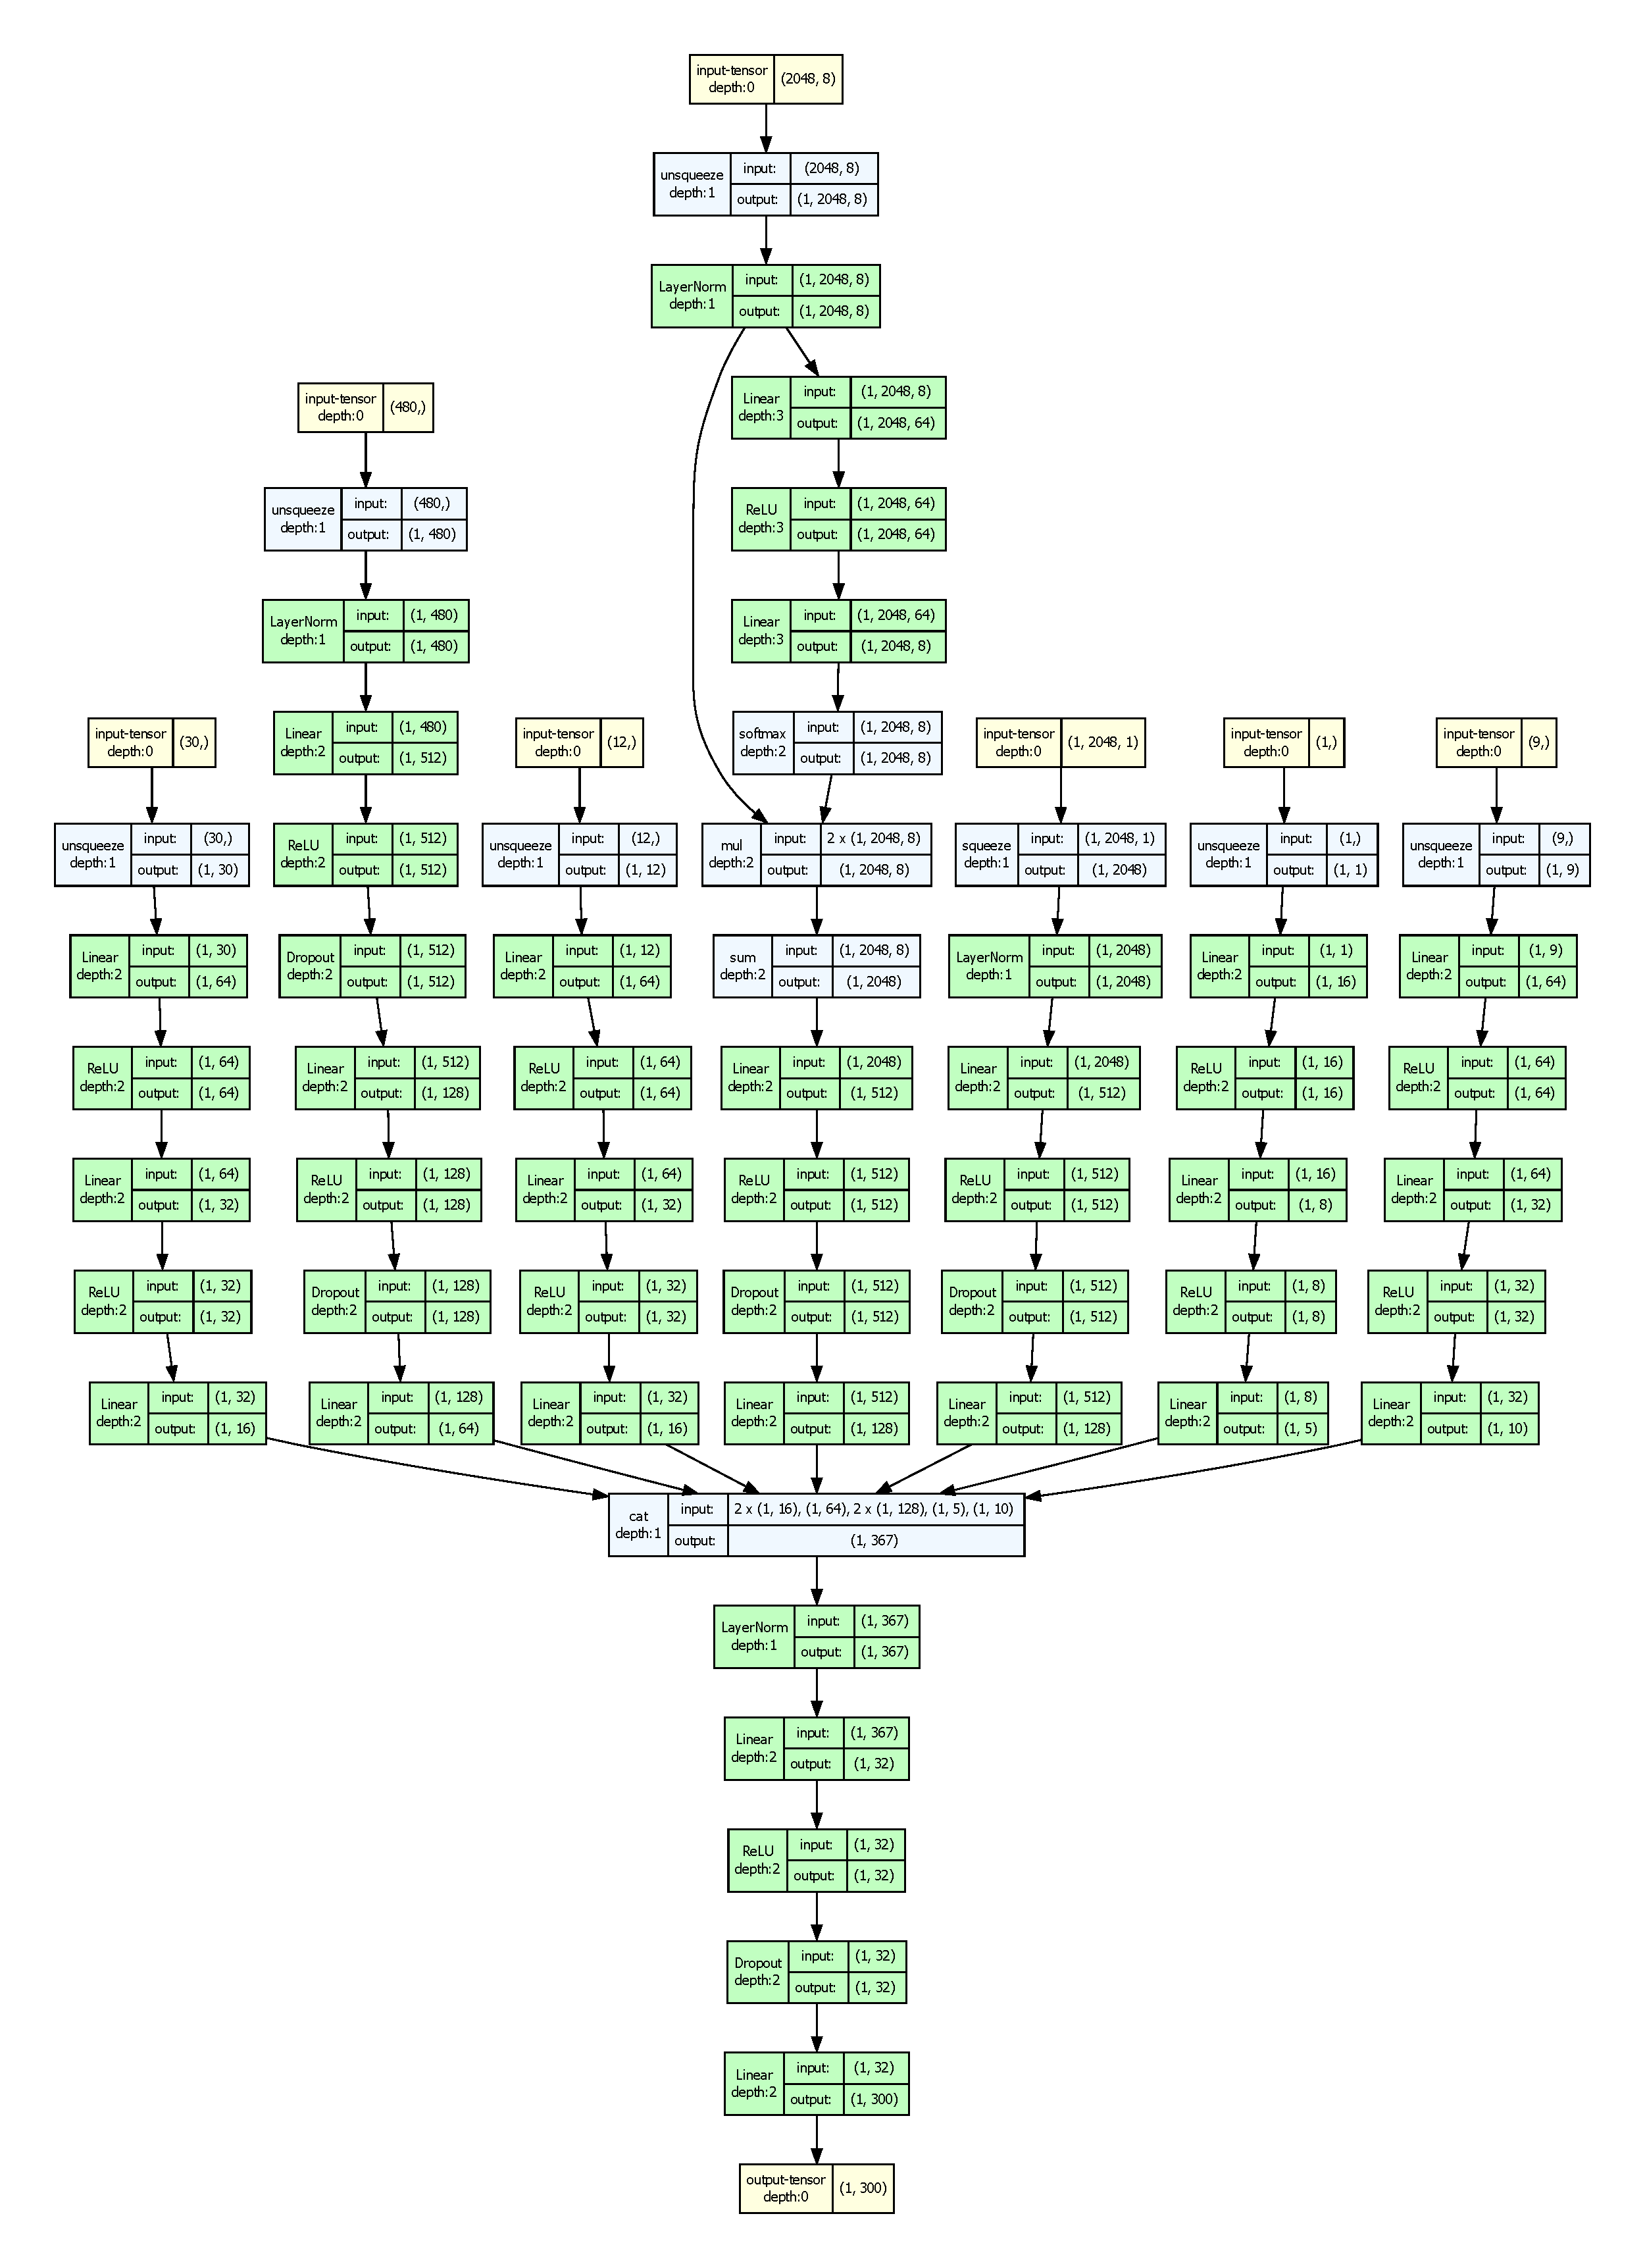
\includegraphics[keepaspectratio,
				width=\paperwidth,
				height=\paperheight]{media/modelArchitectureSeparateTails_complete}
			};
		\end{tikzpicture}
	\end{frame}
}